\documentclass[10pt,conference,compsocconf]{IEEEtran}

\usepackage{hyperref}
\usepackage{graphicx}	% For figure environment
\usepackage[section]{placeins}
% \usepackage{natbib}

\begin{document}
\title{Effect of Dataset Size on Convolutional Models for Building Classification}

\author{
  Francisco, Abhi, Cary\\
  \textit{EPFL, Lausanne, Switzerland}
}

\maketitle

\begin{abstract}
 The Torchvision library offers a wide variety of models for addressing different tasks, including: image classification, pixelwise semantic segmentation, object detection, instance segmentation, person keypoint detection and video classification. Among these models, many state of the art deep learning models can be found already trained on large datasets. This project focuses on using Torchvision models to classify various types of building  for Civil Engineering research. However, when identifying characteristics buildings there is no large labeled database of labeled images, and manually labeling costs much time and resources. This raises the question, of how many samples are needed to sufficiently train a model given limited resources and labeled images? This project explores various data collection and manipulation methods and the effect it had on the resulting classification models. As machine learning is being used more widely across disciplines, large generic datasets most likely will not suffice and knowing how much data is needed for sufficient results is valuable to the success of machine learning.
\end{abstract}

\section{Introduction}
For the purpose of collecting data of the buildings of Switzerland, together with the \textit{Laboratoire dínformatique et mécanique appliquées à la construction}, we were tasked with capturing images of of buildings in Zurich and saving their locations and characteristics. Data was collected using the Google Street-View API and several methods were attempted to manipulate and transform the data sufficiently for the neural network. Then using classification models, certain characteristics were extracted from the images. The building classifciation was broken down into 3 steps, and three corresponding neural net models. The first task was detecting the buildings in an image. The second step was distinguishing openings (windows, doors, etc.) on a building to calculate the opening to façade ratio, a highly important characteristic in determing the type of building. The third step was classifying the buildings based on the materials there were made of.  We have chosen for these tasks:
\begin{itemize}
    \item Faster R-CNN ResNet-50 FPN \cite{DUMMY:1} to extract the buildings from Google Street-View.
    \item DeepLabV3 ResNet101 \cite{DUMMY:1} to differentiate openings on the facade.
    \item ResNet-50 \cite{DUMMY:1} to classify the materials on the facade.
\end{itemize}
Since this project consisted of characterizing buildings with specific characteristics there was no pretrained model or prexisting labeled dataset. Therefore, tools for continuosly sampling images from Google Street-view and an image labeling application was created. Labeling images is arduous task that had to be done by hand, but many labeled samples are necessary to train deep learning models. For this reason, we have studied the effect on the efficacy of the models as the dataset they are trained on increased.

\section {Data Collection}
A large portion of this project was data collection and refinement for the machine learning models. The first image generator simply pulled random images of buildings in Zurich from the Google Street-view API. This method was quick however it gave images that would make it more difficult for the neural net. Buildings appeared from different angles and distortions. In addition, since one goal was to capture the opening to façade ratio, it did not make sense to capture only part of the building since different parts of the building might have disproportional opening to façade ratios, and just the part that is captured is not representative of the entire building. 

To combat this problem, we focused more on how to get the image to the complete building. The Google Street-view API allows one to query an image by location, heading, field of view, and a few other parameters. The API was queried at the same location with various headings such that the camera was panned around a fixed point, creating a panorama. The image was then divided to see each side of the road (180 degrees) individually. As shown in figure \ref{fig:pano1}, this resulting image had some distortion and although it covered the entire building, it might have misled the neural network. This also suffers from the original problem; it captures many different angles of the buildings which could mess up the opening to façade ratio. When looking at a building from an angle, the windows in the front, closer to the observer, are bigger and would count for a larger percentage of the building. This panorama also took about 50 images to complete, which is time consuming and computationally costly. Another simpler panorama algorithm was used to produce an image using only 3 consecutive images. The result, shown in figure \label{fig:pano2}, has much more distortion then before. 

\begin{figure}[h!]
  \centering
  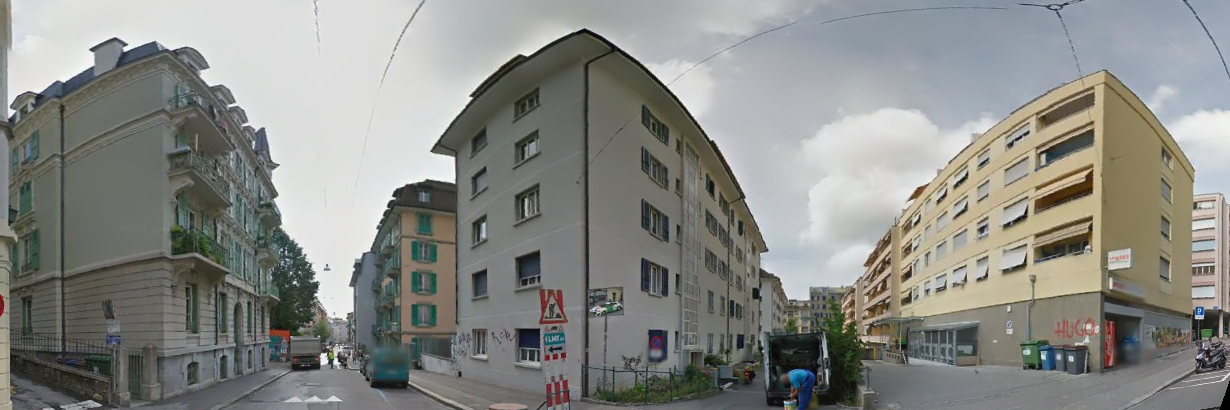
\includegraphics[width=\columnwidth, height=30mm]{panorama_example.png}
  \vspace{-5mm}
  \caption{The panoramic output has a much larger field of view and allows much more information to be captured, however in 2d the façade of the building is distorted and might affect the opening to façade ratio. Additionally, this higher quality required 50 separate images from the Google Street-view API.}
  \label{fig:pano1}
\end{figure}


\begin{figure}[h!]
  \centering
  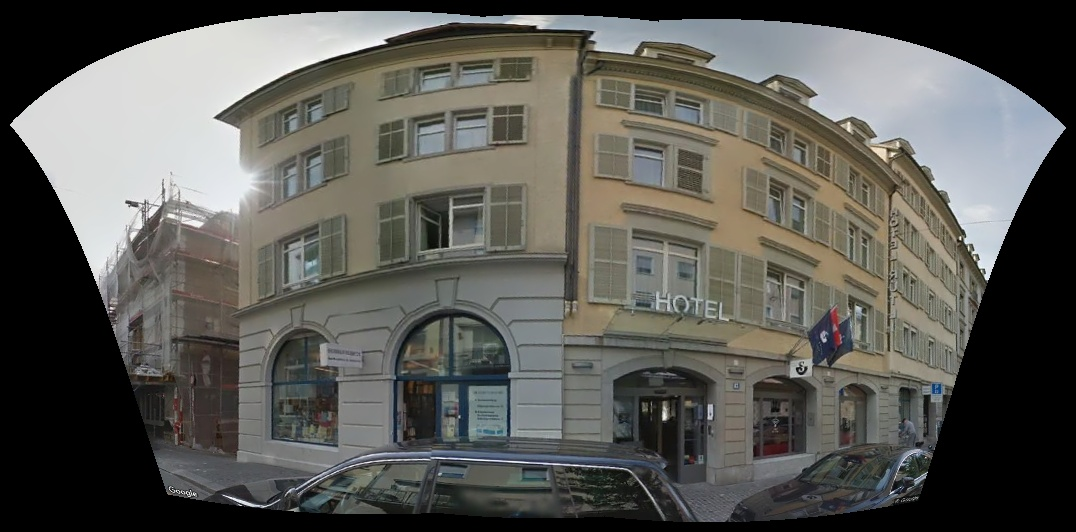
\includegraphics[ height=30mm]{panorama2_less_imgs.png}
  \vspace{-5mm}
  \caption{This is a quick stitch that takes significantly less images (only 3 images) and the image is facing the buildings directly, however, it has some distortion.}
  \label{fig:pano2}
\end{figure}

The second and more effective solution to generating sufficient images was to use a preexisting database of coordinates of buildings in Zurich, provided by the \textit{Laboratoire dínformatique et mécanique appliquées à la construction}. This database provided approximately the longitude and latitude values for the center of the midpoint of each building. Using this coordinate, the Google Roads API was used. It contained a snap-to-road function which inputs any coordinate pair and returns the coordinates to the nearest road. Then the Google Street view API was used to get the image of the building at that coordinate. Now the image could be guaranteed to be facing the building straight on, by calculating the desired heading of the camera to be perpendicular to the road and the building. This direction can be calculated by taking the difference from building coordinates to the corresponding snapped road coordinates and using basic trigonometry to calculate the angle relative to North that the building was at, since North corresponded to zero degrees heading in the Google Street-view API queries.  A good example is shown in \ref{fig:finalImg}.

\begin{figure}[h!]
  \centering
  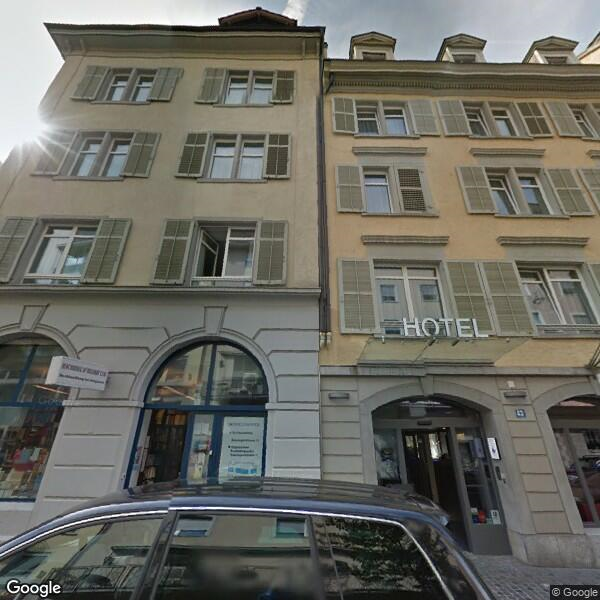
\includegraphics[height=30mm]{final_img_example.png}
  \vspace{-5mm}
  \caption{In the regular view, less of each building is captured however the image is taken perpendicular to the façade, which would in theory provide a more accurate façade to opening ratio.}
  \label{fig:finalImg}
\end{figure}

Although most of the images are captured perpendicular to the building there are still some issues. Images from the Google API taken from the sidewalk do not have a fixed heading of 0 corresponding to North as do those taken from the road, therefore those images are still not facing directly towards the building after the heading calculation. Also, the database of buildings contained more buildings then the Google Roads API, so there were many times where different buildings would snap to the same nearest road or calling the Google Street view API would return the same image. The data generator was later adjusted so that repeated pictures were ignored. In addition, some of the images are blocked by trees, road signs, construction, etc. These cases are somewhat unavoidable and, as in any machine learning problem, not all the data will be perfect, there is always some noise that the model must learn to handle.


\section{Data augmentation}
\label{sec:PreCond}
We used different tactics to increase the dataset size:
\begin{itemize}
    \item Noise addition
    \item Rotate the images between 0 and 15 degrees
    \item Cropping 0 to 10 percent of the images
    \item Vertical axis mirroring
\end{itemize}

\section{Nerual Network Model Selections}


\subsection{Faster R-CNN ResNet-50 FPN}
Object detection behaviour as the dataset increases comparing with and without data augmentation.
\begin{figure}[h!]
  \centering
  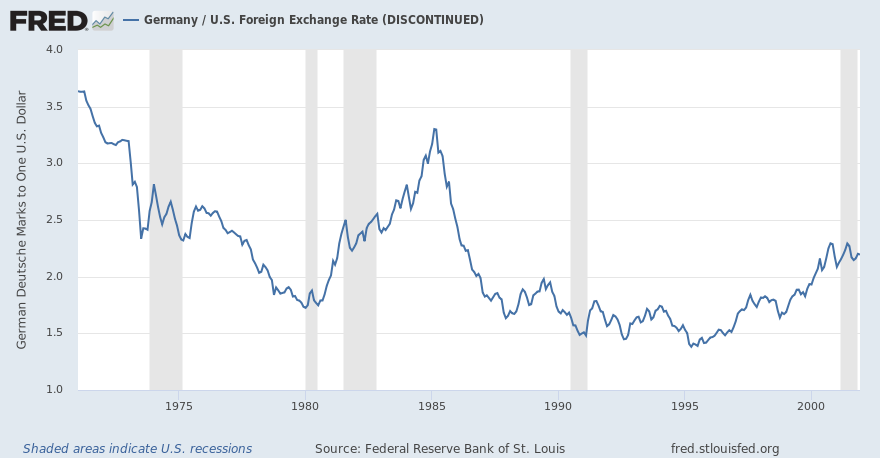
\includegraphics[width=\columnwidth, height=30mm]{download.png}
  \vspace{-5mm}
  \caption{Placeholder}
  \label{fig:first}
\end{figure}

\subsection{DeepLabV3 ResNet101}
Image segmentation behaviour as the dataset increases comparing with and without data augmentation.
\begin{figure}[h!]
  \centering
  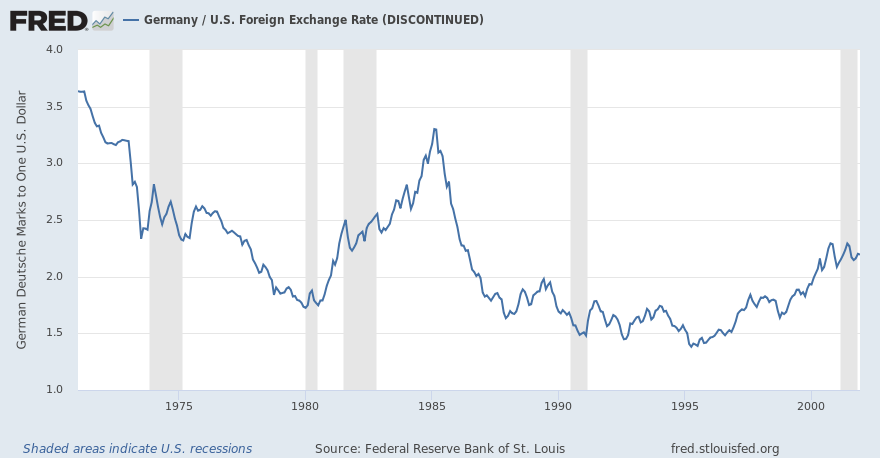
\includegraphics[width=\columnwidth, height=30mm]{download.png}
  \vspace{-5mm}
  \caption{placeholder}
  \label{fig:second}
\end{figure}

\subsection{ResNet-50}
Image classificator behaviour as the dataset increases comparing with and without data augmentation.
\begin{figure}[h!]
  \centering
  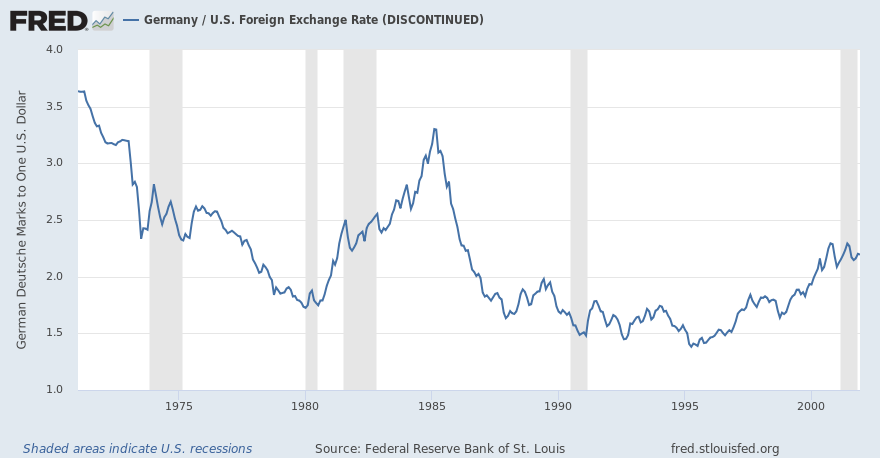
\includegraphics[width=\columnwidth, height=30mm]{download.png}
  \vspace{-5mm}
  \caption{Placeholder}
  \label{fig:third}
\end{figure}

\section{Final Pipeline}
In order to allow for smooth reproducability, a pipeline was created to interface all the relevant commands for this project including data production, labeling, training and testing. The first step is to sample images from the Google APIs. This will pull images store them in the resources/unlabeled/ directory. The data production pipeline keeps track of how many images are produced in a text file, so that the next time data is produced it does not repeat images it has already downloaded. Simultaneous to the image production, the coordinates for each building and corresponding snapped road image are saved externally in csv file in the same directory where the images are produced.  

The next step is to run the labeler. This runs an application that allows the user to either outline bounding boxes of building or paint openings on the façade of the building. An example of the labeler is shown in \ref{fig:labeler} As images are being labeled, they are automatically moved from the unlabed to the labeled folder and in the resources directory. At the same time the labeled information, such as the location of the bounding boxes, or the locations of the painted pixels, is stored in a corrsponding data.csv file. 

\begin{figure}[h!]
  \centering
  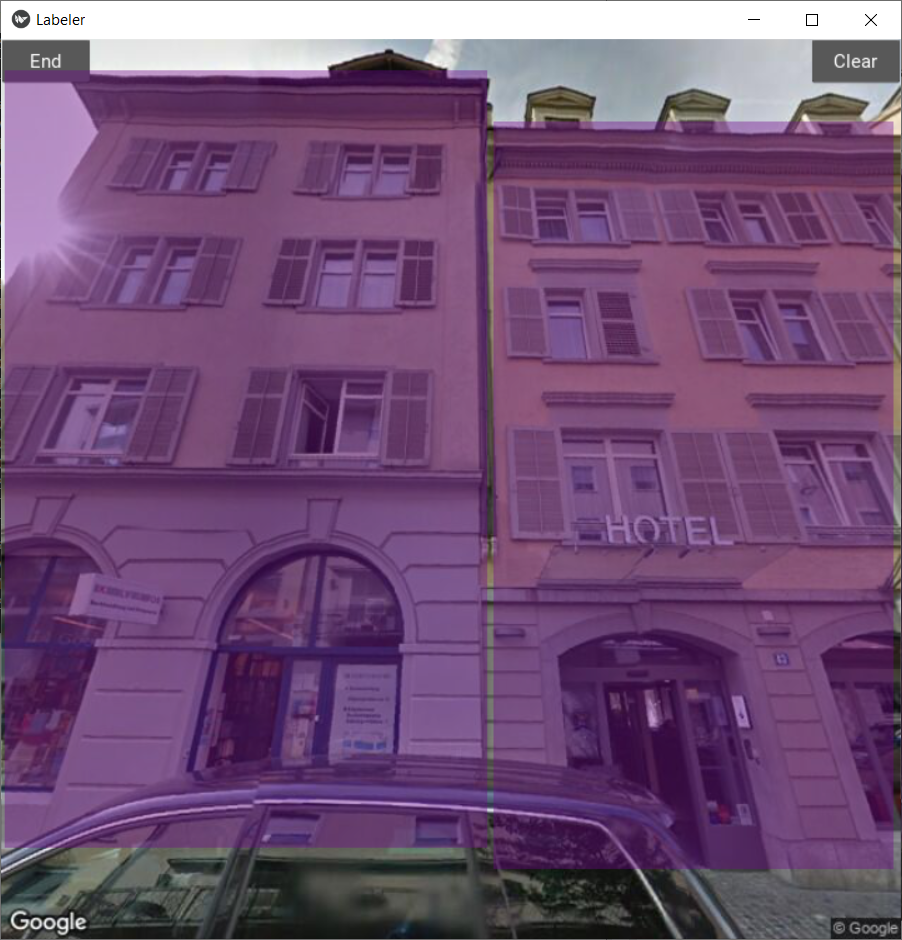
\includegraphics[height=30mm]{labeler.png}
  \vspace{-5mm}
  \caption{This labeling application was created specifically for this project. This image shows the object detection labelers which allows a user to click and drag open a bounding box around the buildings.}
  \label{fig:lebeler}
\end{figure}

After labeling the desired amount of images, the user can run the train command and let the program train for as many hours as needed. It is recommended to use a high performance computer for traning. The training script will automatically detect and use any available GPU to maximize performance and it will periodically conduct tests against unseen samples and store the results. 

Finally, after sufficient training the user can test the trained models on their own data. They simply have to provide a path to the directory where the images are located and the command will return corresponding models output. For example, if the user the gave an image with a set of buildings and ran the building detection model, the testing command would return an array representing the bounding boxes of each building detected.

More informoation, on how to use this project can be found in the corresponding docstring documentation and readMe file. The extensive documentation and focus on reproducability was done to allow further extensions and research by the  \textit{Laboratoire dínformatique et mécanique appliquées à la construction} and any further interested researcher.

\section{Summary}
Summary of each model's results. Comparison between each model's results and hypothesis of the reasons why they happen. 

\section*{Acknowledgements}
We would like to acknowledge the host lab for our prject \textit{Laboratoire dínformatique et mécanique appliquées à la construction}, which provided many resources including the building database of Zurich and a meeting space. In addition, we would like to personally thank our project mentor Alireza Khodaverdian for the advice and guidance throughout the course of this project. Finally, we would like to acknowledge the ML CS-433 Course professors and staff for giving us the freedom and support in conducting this project.

\bibliographystyle{IEEEtran}
\bibliography{literature}

\end{document}
